\documentclass[../template]{subfiles}

\begin{document}
\section{Flusso a costo massimo}
\begin{center}
    \begin{tikzpicture}[rotate=180]
        \Vertices[unit=1.5]{circle}{S, 1, 2, D, 3, 4}
        \Edge(1)(2)
        \Edge(S)(3)
        \Edge(S)(4)
        \Edge(1)(4)
        \Edge(4)(2)
        \Edge(1)(3)
        \Edge(2)(D)
        ;
    \end{tikzpicture}
\end{center}
Quando in un grafo di flusso voglio calcolare la massima trasmissione possibile tra un nodo sorgente $S$ ed un nodo destinazione $D$.
Il resto dei nodi della rete prende il nome di intermedio, ed hanno una capacità limitata $c_{ij}$ che rappresenta la quantità massima
di flusso inviabile attraverso l'arco.
\subsubsection{Taglio a costo minimo}
Si consideri $U \subset V$ tale che $S \in U$ e  $D \notin U$.
L'insieme di archi $S_U = \{(i, j) \in A : i \in U, j \notin U\}$ ovvero gli archi con il un solo estremo in $U$, è
detto taglio della rete.

\vspace{10pt}
\noindent
Ad un taglio è associabile anche un costo, pari alla somma delle capacità del taglio:
\[
    C(S_U) = \sum_{(i, j) \in S_U} c_{ij}
\]
NOTA: Dalla sorgente alla destinazione non è possibile inviare una quantità di prodotto superiore alla capacità di taglio.
Quindi il taglio a costo minimo indica il bottleneck della rete, ovvero la quantità massima di prodotto da sorgente a destinazione.
L'algoritmo di risoluzione del flusso a costo massimo è anche la soluzione al problema del taglio a costo minimo.

\subsection{Procedura di soluzione}
Partire da un flusso ammissibile, $\bar{X} = (\bar{x}_{ij})_{(i, j) \in A}$ ed un cammino orientato $S = q_0 \to q_1 \to \dots \to q_{r} \to q_{r+1} = D$,
privo di archi saturi.
\\
In questo caso $\bar{X}$ non è ottimo, dato che posso ancora inviare una quantità $\Delta = \min_{i=0\dots r} [c_{q_i, q_{i+1}} - \bar{x}_{q_i, q_{i+1}]}$ di prodotto senza violare i vincoli di capacità degli archi.
Sommando $\Delta$ otteniamo un cammino $P$ da $S$ a $D$ contenente almeno un arco saturo.

Definiamo un nuovo grafo orientato $G(\bar{X}) = (V, A(\bar{X}))$, detto grafo associato al flusso $\bar{X}$.
Il nuovo grafo ha gli stessi nodi della rete originaria ed ha il seguente insieme di archi
$A_f$ (archi forward) archi in $P$ non saturi, $A_b$ (archi backward) sono tutti gli archi della rete con $x_{ij} > 0$ (stanno inviando prodotto),
rivolti in orientamento opposto.

Supponiamo che esista un cammino orientato $P$ da $S$ a $D$ in $G(\bar{X})$.
Per ogni arco $(i, j)$ del cammino, calcoliamo il seguente valore:
\[
    \alpha_{ij} =
    \begin{cases}
        c_{ij} - \bar{x}_{ij} &\text{se}\quad (i, j) \in A_f (\bar{X}) \cap P\\
        x_{ji}                &\text{se}\quad (i, j) \in A_{b}(\bar{X}) \cap P
    \end{cases}
\]
Note: $\alpha_{ij}$ indica la quantità di prodotto che si può rispedire indietro lungo l'arco, i.e. di quanto è possibile ridurre il flusso lungo l'arco $(j, i)$.
\\
Una volta calcolati i coefficienti $\alpha_{ij}$, definisco
\[
    \Delta = \min_{(i, j) \in P} \alpha_{ij}
\]
Note: Sottraendo questa quantità $\Delta$ non è mai possibile avere valori di flusso negativi.
\\
Ed aggiorno i flussi $\bar{x}_{ij}$ nel modo seguente:
\[
    \bar{x}_{ij} =
    \begin{cases}
        \bar{x}_{ij} + \Delta & \text{se} \quad (i, j) \in A_f(\bar{X}) \cap P \\
        \bar{x}_{ij} - \Delta & \text{se} \quad (j, i) \in A_b(\bar{X}) \cap P\\
        \bar{x}_{ij} & \text{altrimenti}
    \end{cases}
\]
Note: segue che attraverso tale aggiornamento, sto inviando anche una quantità $\Delta$ in più da sorgente a destinazione.

Diversamente se il grafo $G(\bar{X})$ non contiene cammini orientati da $S$ a $D$, possiamo immediatamente concludere che il flusso $\bar{X}$ è soluzione
ottima del problema di flusso massimo.
Inoltre tutti i nodi raggiungibili dal nodo sorgente con un camino orientato formano l'insieme di nodi che andranno a formare il taglio minimo.

\subsection{Algoritmo di Ford-Fulkerson}
\lstinputlisting{algorithms/ford_fulkerson.py}
\begin{center}
    \begin{minipage}[c]{.4\textwidth}
        \begin{tikzpicture}[EdgeStyle/.style={->}]
            \Vertex[x=0, y=0]{S};
            \Vertex[x=4, y=0]{D};
            \Vertex[x=2, y=1]{1};
            \Vertex[x=2, y=-1]{2};

            \Edge[label=$2/2$](S)(1);
            \Edge[label=$1/2$](1)(D);
            \Edge[label=$1/1$](1)(2);
            \Edge[label=$1/2$](S)(2);
            \Edge[label=$2/2$](2)(D);
            ;
        \end{tikzpicture}
    \end{minipage}
    \begin{minipage}{.47\textwidth}
        \begin{tikzpicture}[EdgeStyle/.style={->}]
            \Vertex[x=0, y=0]{S};
            \Vertex[x=4, y=0]{D};
            \Vertex[x=2, y=1]{1};
            \Vertex[x=2, y=-1]{2};

            \tikzset{EdgeStyle/.append style={color=clr-primary}}
            \Edge(1)(S);
            \Edge(D)(1);
            \Edge(2)(1);
            \Edge(2)(S);
            \Edge(D)(2);

            \tikzset{EdgeStyle/.append style={color=clr-highlight}}
            \tikzset{EdgeStyle/.append style={bend right}}
            \Edge(S)(2);
            \tikzset{EdgeStyle/.append style={bend left}}
            \Edge(1)(D);

            ;
            \node at ([shift={(90:.7cm)}]S){$(S, \infty)$};
            \node at ([shift={(90:.7cm)}]1){$(1, \min(1, 1))$};
            \node at ([shift={(270:.7cm)}]2){$(2, \min(\infty, 2- 1))$};
            \node at ([shift={(270:.7cm)}]D){$(1, \min(1, 2-1))$};
        \end{tikzpicture}
    \end{minipage}
\end{center}

\subsubsection{Teorema}
Se si pone $U = E$, dove $E$ è l'insieme dei nodi etichettati al momento della terminazione dell'algoritmo, si ha che il taglio $S_U$, indotto
da $U$ è soluzione ottima del problema di taglio minimo e il flusso attuale è soluzione ottima del problema di flusso massimo.

\subsubsection{Dimostrazione}
Al momento della terminazione dell'algoritmo si ha $S \in E$ (etichettato al passo 1) e $D \notin E$ (Perché rimosso al passo 3).
Quindi l'insieme $E$ induce effettivamente un taglio.
\\[10pt]
Se il valore di tale taglio coincide con il valore del flusso uscente da $S$, avendo già osservato che il costo di ogni taglio non è inferiore al
valore del flusso massimo, possiamo concludere che esso è il taglio a costo minimo ed il flusso attualmente uscente da $S$ è massimo.
\\[10pt]
Misurando il flusso uscente da $S$, esso coincide con il flusso uscente dai nodi in $E$, che viene spostato verso i nodi nel complemento $\bar{E} = V - E$,
meno il flusso che in senso opposto: da $\bar{E}$ a $E$.
\\[10pt]
Per dimostrare che la quantità di prodotto complessivamente inviata da $S$ a $D$ è pari a:
\[
    \sum_{(i, j) : (i, j) \in A, i \in E, j \in \bar{E}} \bar{x}_{ij} -
    \sum_{(j, i) : (j, i) \in A, i \in E, j \in \bar{E}} \bar{x}_{ji}
\]
osserviamo che si deve avere $\forall (i, j) \in A, i \in E, j\in \bar{E} \bar{x}_{ij} = c_{ij}$. Infatti, per assurdo si supponga che $\exists (i_1, j_1) \in A, i_1 \in E, j_1 \in \bar{E} : \bar{x}_{i_1 j_1} < c_{i_1 j_1}$.
In tal caso $(i_1, j_1) \in A_f(\bar{X})$, ma al passo 2, il nodo $j_1$
dovrebbe essere stato aggiunto ad $E$. Il che contraddice $j_1 \notin E$.

Si deve avere inoltre che $\forall (j, i) \in A, i \in E, j \in \bar{E} \quad \bar{x}_{ji} = 0$, infatti, per assurdo si supponga che esista un $(j_1, i_1) \in A: i_1 \in E, j_1 \in \bar{E}, \bar{x}_{j_1 i_1} > 0$.
In tal caso $(i_1, j_1) \in A_b(\bar{X})$, e quindi al passo 2, sarebbe anch'esso stato aggiunto ad $E$, contraddicendo l'ipotesi.
%0h:46m
\\[10pt]
Sostituendo i valori di queste due osservazioni nella formula precedente,
si ottiene che il valore de flusso è pari al costo del taglio introdotto da $E$:
\[
    \sum_{(i, j) : (i, j) \in A, i \in E, j \in \bar{E}} c_{ij} = C(S_E)
\]
\subsubsection{Complessità dell'algoritmo}
$O(|A||V|^2)$ (se $i$ è scelto tramite un metodo FIFO).
Esistono raffinamenti di questo algoritmo di complessità $O(|V|^3)$.
%0h:55 - cosa succede se Non uso un metodo FIFO
\end{document}
